\documentclass{standalone}
\usepackage{tikz}
\usepackage{pgfplots}
\pgfplotsset{compat=1.18}

\begin{document}
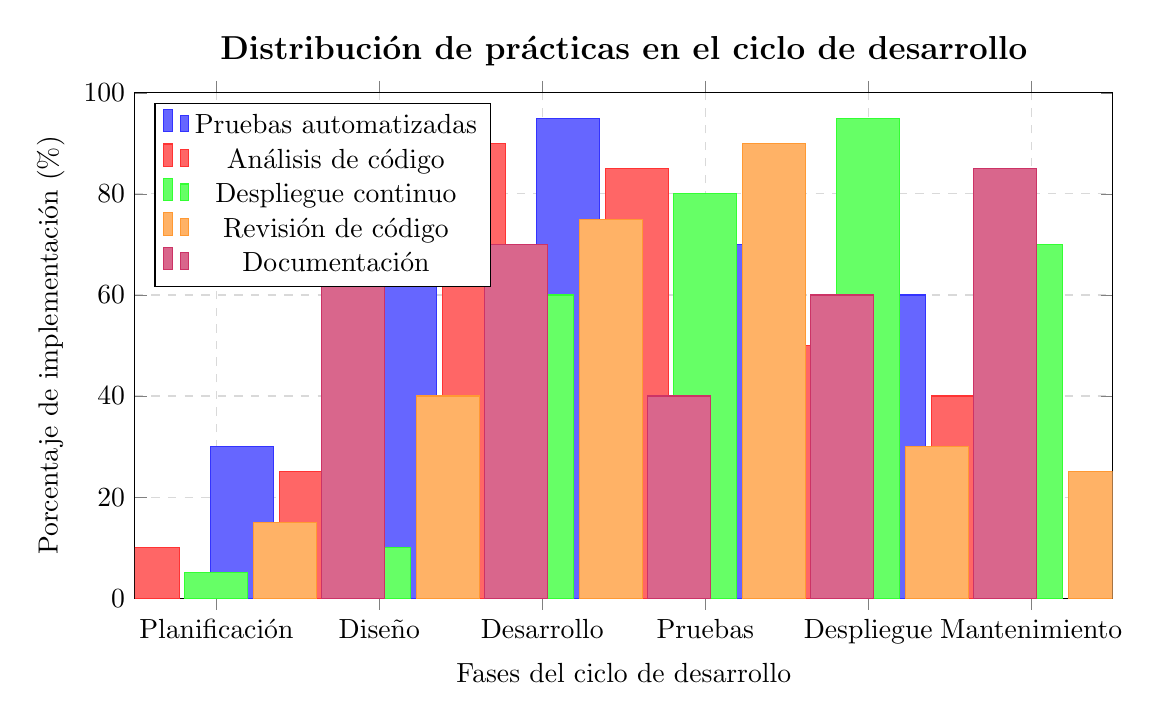
\begin{tikzpicture}
\begin{axis}[
    ybar,
    bar width=0.8cm,
    width=14cm,
    height=8cm,
    ylabel={Porcentaje de implementación (\%)},
    xlabel={Fases del ciclo de desarrollo},
    xtick=data,
    xticklabels={Planificación, Diseño, Desarrollo, Pruebas, Despliegue, Mantenimiento},
    ymin=0,
    ymax=100,
    grid=major,
    grid style={dashed,gray!30},
    legend pos=north west,
    legend style={at={(0.02,0.98)},anchor=north west},
    title={Distribución de prácticas en el ciclo de desarrollo},
    title style={font=\large\bfseries}
]

% Pruebas automatizadas
\addplot[fill=blue!60, draw=blue!80] coordinates {
    (1, 20) (2, 30) (3, 85) (4, 95) (5, 70) (6, 60)
};

% Análisis de código
\addplot[fill=red!60, draw=red!80] coordinates {
    (1, 10) (2, 25) (3, 90) (4, 85) (5, 50) (6, 40)
};

% Despliegue continuo
\addplot[fill=green!60, draw=green!80] coordinates {
    (1, 5) (2, 10) (3, 60) (4, 80) (5, 95) (6, 70)
};

% Revisión de código
\addplot[fill=orange!60, draw=orange!80] coordinates {
    (1, 15) (2, 40) (3, 75) (4, 90) (5, 30) (6, 25)
};

% Documentación
\addplot[fill=purple!60, draw=purple!80] coordinates {
    (1, 80) (2, 70) (3, 40) (4, 60) (5, 85) (6, 90)
};

\legend{Pruebas automatizadas, Análisis de código, Despliegue continuo, Revisión de código, Documentación}

\end{axis}
\end{tikzpicture}
\end{document}
